\documentclass[aspectratio=169,11pt]{beamer}

% TEMA Y COLORES
\usetheme{Madrid}
\usecolortheme{whale}

\definecolor{primaryblue}{RGB}{0,102,153}
\definecolor{accentgreen}{RGB}{0,128,0}
\definecolor{accentorange}{RGB}{204,102,0}
\definecolor{darkgray}{RGB}{64,64,64}

\setbeamercolor{palette primary}{bg=primaryblue,fg=white}
\setbeamercolor{palette secondary}{bg=primaryblue!80,fg=white}
\setbeamercolor{palette tertiary}{bg=primaryblue!60,fg=white}
\setbeamercolor{structure}{fg=primaryblue}
\setbeamercolor{block title}{bg=primaryblue,fg=white}
\setbeamercolor{block body}{bg=primaryblue!10}
\setbeamercolor{block title example}{bg=accentgreen,fg=white}
\setbeamercolor{block body example}{bg=accentgreen!10}
\setbeamercolor{block title alerted}{bg=accentorange,fg=white}
\setbeamercolor{block body alerted}{bg=accentorange!10}

% PAQUETES
\usepackage[utf8]{inputenc}
\usepackage[T1]{fontenc}
\usepackage{amsmath,amssymb}
\usepackage{booktabs}
\usepackage{tikz}
\usepackage{pgfplots}
\usepackage{listings}
\usepackage{multicol}

\pgfplotsset{compat=1.17}
\lstset{literate={ñ}{{\~n}}1 {á}{{\'a}}1 {é}{{\'e}}1 {í}{{\'i}}1 {ó}{{\'o}}1 {ú}{{\'u}}1}
% CÓDIGO PYTHON
\lstdefinestyle{pythonstyle}{
    language=Python,
    basicstyle=\ttfamily\footnotesize,
    keywordstyle=\color{blue}\bfseries,
    stringstyle=\color{red},
    commentstyle=\color{accentgreen}\itshape,
    frame=single,
    breaklines=true,
    showstringspaces=false,
    backgroundcolor=\color{gray!10}
}

% NAVEGACIÓN Y PIE DE PÁGINA
\setbeamertemplate{navigation symbols}{}
\setbeamertemplate{footline}{
    \leavevmode%
    \hbox{%
        \begin{beamercolorbox}[wd=.333333\paperwidth,ht=2.25ex,dp=1ex,center]{author in head/foot}%
            \usebeamerfont{author in head/foot}Matemáticas Financieras
        \end{beamercolorbox}%
        \begin{beamercolorbox}[wd=.333333\paperwidth,ht=2.25ex,dp=1ex,center]{title in head/foot}%
            \usebeamerfont{title in head/foot}Sesión 10
        \end{beamercolorbox}%
        \begin{beamercolorbox}[wd=.333333\paperwidth,ht=2.25ex,dp=1ex,right]{date in head/foot}%
            \usebeamerfont{date in head/foot}\insertframenumber{} / \inserttotalframenumber\hspace*{2ex}
        \end{beamercolorbox}}%
    \vskip0pt%
}

\title[Sesión 10]{Valuación de Acciones e Integración}
\subtitle{Modelos de dividendos y repaso general}
\author{Matemáticas Financieras}
\institute{Valor del Dinero en el Tiempo}
\date{Semana 5 | Clase 2 | Duración: 1h 50min}

\begin{document}

% ===========================================
% SECCIÓN 1: PORTADA Y CONTENIDO
% ===========================================

\begin{frame}
    \titlepage
\end{frame}

\begin{frame}{Contenido de la Sesión}
    \tableofcontents
\end{frame}

% ===========================================
% SECCIÓN 2: INTRODUCCIÓN
% ===========================================
\section{Introducción}

\begin{frame}{Conexión con la Sesión Anterior}
    \begin{block}{Sesión 9: VPN y TIR}
        Evaluamos proyectos de inversión con flujos variables:
        \[
        VPN = \sum_{t=1}^{n} \frac{CF_t}{(1+r)^t} - I_0
        \]
    \end{block}

    \pause
    \vspace{0.3cm}

    \begin{alertblock}{Hoy: Valuación de Acciones}
        Las acciones generan flujos (dividendos) que pueden pagarse \textbf{indefinidamente}.

        Aplicaremos conceptos de perpetuidades (Sesión 6) y descuento de flujos para valuar acciones.
    \end{alertblock}
\end{frame}

\begin{frame}{Objetivos de Aprendizaje}
    Al finalizar esta sesión, serás capaz de:
    \begin{enumerate}
        \item Aplicar el modelo de descuento de dividendos (DDM)
        \item Usar el modelo de Gordon para acciones con crecimiento constante
        \item Valuar acciones con múltiples etapas de crecimiento
        \item Interpretar múltiplos de valuación (P/E, P/B)
        \item Integrar todos los conceptos del curso en un caso práctico
        \item Resolver problemas que combinan múltiples temas
    \end{enumerate}
\end{frame}

\begin{frame}{El Valor Intrínseco de una Acción}
    \begin{block}{Principio Fundamental}
        El valor de una acción es el \textbf{valor presente} de todos los flujos futuros que recibirá el inversionista.
    \end{block}

    \pause
    \vspace{0.3cm}

    \textbf{¿Qué flujos recibe un accionista?}
    \begin{enumerate}
        \item \textbf{Dividendos:} Pagos periódicos de las utilidades
        \item \textbf{Precio de venta:} Al vender la acción en el futuro
    \end{enumerate}

    \pause
    \vspace{0.3cm}

    \begin{exampleblock}{Insight clave}
        El precio de venta futuro también depende de los dividendos futuros.

        Por lo tanto, el valor de una acción es el VP de \textbf{todos los dividendos futuros}.
    \end{exampleblock}
\end{frame}

% ===========================================
% SECCIÓN 3: MODELO DE DESCUENTO DE DIVIDENDOS
% ===========================================
\section{Modelo de Descuento de Dividendos (DDM)}

\begin{frame}{El Modelo General de Dividendos}
    \begin{block}{Dividend Discount Model (DDM)}
        \[
        \boxed{P_0 = \sum_{t=1}^{\infty} \frac{D_t}{(1+r)^t}}
        \]
        donde:
        \begin{itemize}
            \item $P_0$ = Precio actual de la acción
            \item $D_t$ = Dividendo esperado en el período $t$
            \item $r$ = Tasa de rendimiento requerida
        \end{itemize}
    \end{block}

    \pause
    \vspace{0.3cm}

    \begin{alertblock}{Desafío}
        Necesitamos estimar dividendos infinitos. Usamos supuestos simplificadores sobre el patrón de crecimiento.
    \end{alertblock}
\end{frame}

\begin{frame}{Caso 1: Dividendos Constantes (Perpetuidad)}
    Si los dividendos son constantes para siempre:

    \pause
    \begin{block}{Precio con Dividendos Constantes}
        \[
        \boxed{P_0 = \frac{D}{r}}
        \]
    \end{block}

    \pause
    \vspace{0.3cm}

    \begin{exampleblock}{Ejemplo: Acciones Preferentes}
        Una acción preferente paga \$5 de dividendo anual perpetuamente. Si la tasa requerida es 8\%, el precio es:
        \[
        P_0 = \frac{5}{0.08} = \$62.50
        \]
    \end{exampleblock}
\end{frame}

\begin{frame}{Caso 2: Crecimiento Constante (Modelo de Gordon)}
    Si los dividendos crecen a tasa constante $g$ perpetuamente:

    \pause
    \begin{block}{Modelo de Gordon (Gordon Growth Model)}
        \[
        \boxed{P_0 = \frac{D_1}{r - g} = \frac{D_0(1+g)}{r - g}}
        \]
        donde:
        \begin{itemize}
            \item $D_0$ = Dividendo más reciente (ya pagado)
            \item $D_1$ = Dividendo esperado el próximo período
            \item $g$ = Tasa de crecimiento de dividendos
            \item $r$ = Tasa de rendimiento requerida ($r > g$)
        \end{itemize}
    \end{block}

    \pause
    \vspace{0.3cm}

    \textbf{Recordatorio:} Ya derivamos esta fórmula en la Sesión 6 (perpetuidad creciente).
\end{frame}

\begin{frame}{Ejemplo: Modelo de Gordon}
    \begin{block}{Problema}
        Una empresa pagó un dividendo de \$2.00 por acción. Se espera que los dividendos crezcan 5\% anual indefinidamente. Si la tasa requerida es 12\%, ¿cuál es el precio justo?
    \end{block}

    \pause
    \vspace{0.3cm}

    \textbf{Datos:}
    \begin{itemize}
        \item $D_0 = \$2.00$ (dividendo recién pagado)
        \item $g = 5\%$
        \item $r = 12\%$
    \end{itemize}

    \pause
    \textbf{Solución:}
    \begin{align*}
        D_1 &= D_0 \times (1+g) = 2.00 \times 1.05 = \$2.10 \\[0.2cm]
        P_0 &= \frac{D_1}{r - g} = \frac{2.10}{0.12 - 0.05} = \frac{2.10}{0.07} = \$30.00
    \end{align*}
\end{frame}

\begin{frame}{Interpretación del Modelo de Gordon}
    \textbf{Rendimiento total = Rendimiento por dividendo + Ganancia de capital}

    \pause
    \vspace{0.3cm}

    \begin{align*}
        r &= \frac{D_1}{P_0} + g \\[0.2cm]
        12\% &= \frac{2.10}{30} + 5\% = 7\% + 5\%
    \end{align*}

    \pause
    \vspace{0.3cm}

    \begin{exampleblock}{Componentes del rendimiento}
        \begin{itemize}
            \item \textbf{Dividend yield} ($D_1/P_0$): 7\% -- ingreso por dividendos
            \item \textbf{Ganancia de capital} ($g$): 5\% -- apreciación del precio
        \end{itemize}
    \end{exampleblock}
\end{frame}

\begin{frame}{Sensibilidad del Modelo de Gordon}
    \begin{center}
        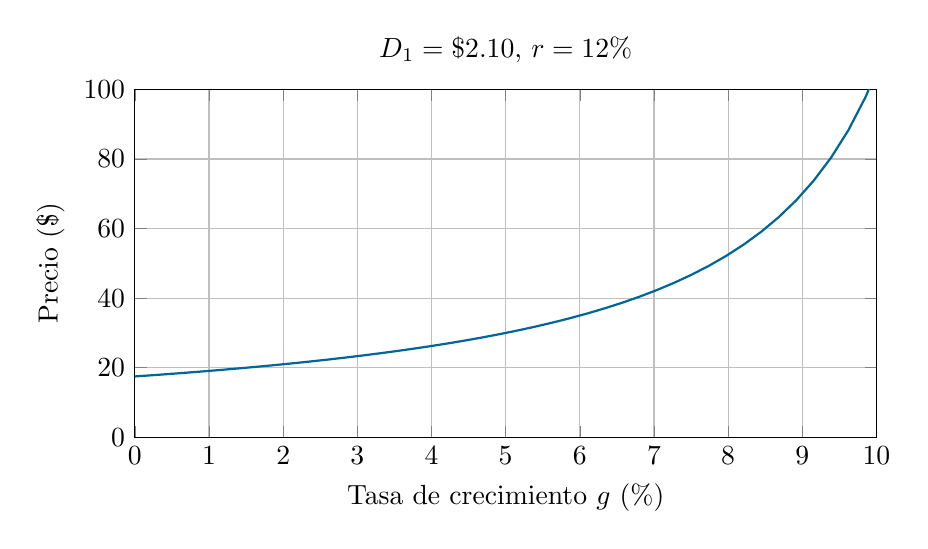
\begin{tikzpicture}
            \begin{axis}[
                xlabel={Tasa de crecimiento $g$ (\%)},
                ylabel={Precio (\$)},
                xmin=0, xmax=10,
                ymin=0, ymax=100,
                grid=major,
                width=11cm,
                height=6cm,
                title={$D_1 = \$2.10$, $r = 12\%$}
            ]
            \addplot[color=primaryblue, thick, domain=0:11.5, samples=50]
                {2.10/(0.12 - x/100)};

            \addplot[color=red, dashed] coordinates {(12,0) (12,100)};
            \end{axis}
        \end{tikzpicture}
    \end{center}

    El precio es muy sensible a $g$, especialmente cuando se acerca a $r$.
\end{frame}

\section{Modelos de Múltiples Etapas}

\begin{frame}{¿Por qué Múltiples Etapas?}
    \begin{alertblock}{Limitación del Modelo de Gordon}
        Supone crecimiento constante \textbf{para siempre}, lo cual es irrealista para muchas empresas.
    \end{alertblock}

    \pause
    \vspace{0.3cm}

    \textbf{Patrones de crecimiento más realistas:}
    \begin{itemize}
        \item Empresas jóvenes: alto crecimiento inicial, luego estabilización
        \item Empresas maduras: crecimiento estable o declinante
        \item Empresas cíclicas: crecimiento variable
    \end{itemize}

    \pause
    \vspace{0.3cm}

    \begin{exampleblock}{Solución}
        Dividir el horizonte en etapas con diferentes tasas de crecimiento.
    \end{exampleblock}
\end{frame}

\begin{frame}{Modelo de Dos Etapas}
    \begin{block}{Estructura}
        \begin{enumerate}
            \item \textbf{Etapa 1 (años 1 a T):} Crecimiento alto $g_1$
            \item \textbf{Etapa 2 (año T+1 en adelante):} Crecimiento estable $g_2$
        \end{enumerate}
    \end{block}

    \pause
    \vspace{0.3cm}

    \begin{block}{Fórmula}
        \[
        \boxed{P_0 = \sum_{t=1}^{T} \frac{D_0(1+g_1)^t}{(1+r)^t} + \frac{P_T}{(1+r)^T}}
        \]
        donde:
        \[
        P_T = \frac{D_{T+1}}{r - g_2} = \frac{D_0(1+g_1)^T(1+g_2)}{r - g_2}
        \]
    \end{block}
\end{frame}

\begin{frame}{Ejemplo: Modelo de Dos Etapas}
    \begin{block}{Problema}
        Dividendo actual: \$1.50. Crecimiento 20\% por 3 años, luego 4\% perpetuamente. Tasa requerida: 15\%.
    \end{block}

    \pause
    \vspace{0.2cm}

    \textbf{Paso 1: Dividendos de la etapa de alto crecimiento}
    \begin{align*}
        D_1 &= 1.50 \times 1.20 = \$1.80 \\
        D_2 &= 1.80 \times 1.20 = \$2.16 \\
        D_3 &= 2.16 \times 1.20 = \$2.59
    \end{align*}

    \pause
    \textbf{Paso 2: Precio terminal al final del año 3}
    \begin{align*}
        D_4 &= 2.59 \times 1.04 = \$2.70 \\
        P_3 &= \frac{2.70}{0.15 - 0.04} = \frac{2.70}{0.11} = \$24.52
    \end{align*}
\end{frame}

\begin{frame}{Ejemplo: Modelo de Dos Etapas (Continuación)}
    \textbf{Paso 3: Valor presente de todos los flujos}

    \pause
    \begin{align*}
        P_0 &= \frac{1.80}{1.15} + \frac{2.16}{1.15^2} + \frac{2.59 + 24.52}{1.15^3} \\[0.2cm]
        &= \frac{1.80}{1.15} + \frac{2.16}{1.3225} + \frac{27.11}{1.5209} \\[0.2cm]
        &= 1.57 + 1.63 + 17.83 = \$21.03
    \end{align*}

    \pause
    \vspace{0.3cm}

    \textbf{El precio justo es \$21.03}

    \begin{itemize}
        \item VP de dividendos años 1-3: \$1.57 + \$1.63 + \$1.70 = \$4.90
        \item VP del precio terminal: \$16.13
    \end{itemize}
\end{frame}

% ===========================================
% SECCIÓN 4: MÚLTIPLOS DE VALUACIÓN
% ===========================================
\section{Múltiplos de Valuación}

\begin{frame}{Valuación por Múltiplos}
    \begin{block}{Idea Central}
        Comparar el precio de una acción con alguna métrica fundamental (utilidades, valor en libros, ventas) usando empresas comparables.
    \end{block}

    \pause
    \vspace{0.3cm}

    \textbf{Múltiplos comunes:}
    \begin{itemize}
        \item \textbf{P/E (Price to Earnings):} Precio / Utilidad por acción
        \item \textbf{P/B (Price to Book):} Precio / Valor en libros por acción
        \item \textbf{P/S (Price to Sales):} Precio / Ventas por acción
        \item \textbf{EV/EBITDA:} Valor empresa / EBITDA
    \end{itemize}

    \pause
    \vspace{0.3cm}

    \begin{alertblock}{Valuación relativa}
        Si empresas similares tienen P/E de 15x y nuestra empresa gana \$3/acción, entonces:
        $P_{estimado} = 15 \times \$3 = \$45$
    \end{alertblock}
\end{frame}

\begin{frame}{El Múltiplo P/E (Price to Earnings)}
    \begin{block}{Definición}
        \[
        P/E = \frac{\text{Precio por acción}}{\text{Utilidad por acción (UPA)}}
        \]
    \end{block}

    \pause
    \vspace{0.3cm}

    \textbf{Relación con el Modelo de Gordon:}

    Si $D_1 = UPA \times \text{payout ratio} = UPA \times b$:
    \begin{align*}
        P_0 &= \frac{UPA \times b}{r - g} \\[0.2cm]
        \frac{P_0}{UPA} &= \frac{b}{r - g}
    \end{align*}

    \pause
    \begin{block}{P/E Justificado}
        \[
        \boxed{\frac{P}{E} = \frac{b}{r - g}}
        \]
        donde $b$ = ratio de pago de dividendos
    \end{block}
\end{frame}

\begin{frame}{Interpretación del P/E}
    \textbf{¿Qué significa un P/E alto?}

    \pause
    \vspace{0.3cm}

    \begin{columns}
        \begin{column}{0.48\textwidth}
            \textbf{P/E alto puede indicar:}
            \begin{itemize}
                \item Expectativas de alto crecimiento ($g$ alto)
                \item Bajo riesgo ($r$ bajo)
                \item Posible sobrevaloración
            \end{itemize}
        \end{column}

        \begin{column}{0.48\textwidth}
            \textbf{P/E bajo puede indicar:}
            \begin{itemize}
                \item Expectativas de bajo crecimiento
                \item Alto riesgo
                \item Posible subvaloración
            \end{itemize}
        \end{column}
    \end{columns}

    \pause
    \vspace{0.5cm}

    \begin{alertblock}{Precaución}
        El P/E debe interpretarse en contexto: industria, ciclo económico, calidad de utilidades.
    \end{alertblock}
\end{frame}

\begin{frame}{Ejemplo: Valuación por P/E}
    \begin{block}{Problema}
        Empresa XYZ tiene UPA de \$4.50. Empresas comparables tienen P/E promedio de 18x. ¿Cuál es el valor estimado de XYZ?
    \end{block}

    \pause
    \vspace{0.3cm}

    \textbf{Solución:}
    \begin{align*}
        P_{estimado} = UPA \times P/E_{comparables} = 4.50 \times 18 = \$81.00
    \end{align*}

    \pause
    \vspace{0.3cm}

    \textbf{Si XYZ cotiza a \$72:}
    \begin{itemize}
        \item P/E actual = $72/4.50 = 16x$
        \item Posiblemente subvaluada vs. comparables
        \item O hay razones para el descuento (menor crecimiento, mayor riesgo)
    \end{itemize}
\end{frame}

% ===========================================
% SECCIÓN 5: CASO INTEGRADOR
% ===========================================
\section{Caso Integrador}

\begin{frame}{Caso: Planificación Financiera Personal}
    \begin{block}{Situación}
        María, 30 años, planea su retiro a los 60 años. Quiere:
        \begin{itemize}
            \item Ahorrar mensualmente durante 30 años
            \item Recibir \$50,000 mensuales (reales) por 25 años de retiro
            \item Tasa real de rendimiento: 5\% anual
        \end{itemize}
        ¿Cuánto debe ahorrar mensualmente?
    \end{block}

    \pause
    \vspace{0.3cm}

    \textbf{Este problema integra:}
    \begin{itemize}
        \item Valor del dinero en el tiempo (Sesión 1-2)
        \item Anualidades (Sesión 5-6)
        \item Tasas reales (Sesión 4)
    \end{itemize}
\end{frame}

\begin{frame}{Caso Integrador: Solución Paso 1}
    \textbf{Paso 1: ¿Cuánto necesita al momento del retiro?}

    \pause
    \vspace{0.3cm}

    Tasa mensual real: $r_m = (1.05)^{1/12} - 1 = 0.407\%$

    Meses de retiro: $n = 25 \times 12 = 300$

    \pause
    \begin{align*}
        PV_{retiro} &= PMT \times \frac{1-(1+r_m)^{-n}}{r_m} \\[0.2cm]
        &= 50,000 \times \frac{1-(1.00407)^{-300}}{0.00407} \\[0.2cm]
        &= 50,000 \times 172.55 = \$8,627,500
    \end{align*}

    \pause
    María necesita \textbf{\$8,627,500} al momento de retirarse.
\end{frame}

\begin{frame}{Caso Integrador: Solución Paso 2}
    \textbf{Paso 2: ¿Cuánto debe ahorrar mensualmente?}

    \pause
    \vspace{0.3cm}

    Meta: $FV = \$8,627,500$

    Meses de ahorro: $n = 30 \times 12 = 360$

    Tasa mensual real: $r_m = 0.407\%$

    \pause
    \begin{align*}
        PMT &= FV \times \frac{r_m}{(1+r_m)^n - 1} \\[0.2cm]
        &= 8,627,500 \times \frac{0.00407}{(1.00407)^{360} - 1} \\[0.2cm]
        &= 8,627,500 \times \frac{0.00407}{3.316} \\[0.2cm]
        &= 8,627,500 \times 0.001228 = \$10,594
    \end{align*}

    \pause
    María debe ahorrar \textbf{\$10,594 mensuales} (en términos reales).
\end{frame}

\begin{frame}{Caso Integrador: Verificación}
    \textbf{Verificación con Python:}

    \vspace{0.3cm}

    \begin{center}
    \begin{tabular}{@{}ll@{}}
        \toprule
        \textbf{Concepto} & \textbf{Valor} \\
        \midrule
        Ahorro mensual & \$10,594 \\
        Total ahorrado (nominal) & \$10,594 $\times$ 360 = \$3,813,840 \\
        Acumulado al retiro & \$8,627,500 \\
        Intereses ganados & \$4,813,660 \\
        Retiro mensual & \$50,000 \\
        Total retirado & \$50,000 $\times$ 300 = \$15,000,000 \\
        \bottomrule
    \end{tabular}
    \end{center}

    \pause
    \vspace{0.3cm}

    \begin{exampleblock}{Poder del interés compuesto}
        María ahorra \$3.8M pero retira \$15M gracias al crecimiento compuesto.
    \end{exampleblock}
\end{frame}

% ===========================================
% SECCIÓN 6: REPASO GENERAL
% ===========================================
\section{Repaso General del Curso}

\begin{frame}{Mapa Conceptual del Curso}
    \begin{center}
        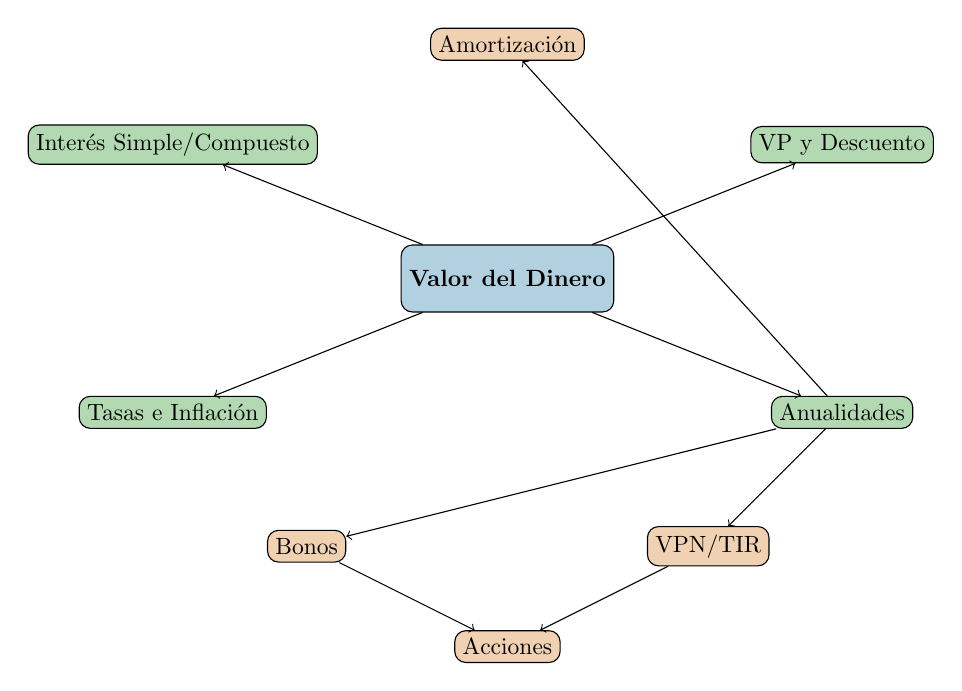
\begin{tikzpicture}[scale=0.85, every node/.style={scale=0.85}]
            % Nodo central
            \node[draw, fill=primaryblue!30, rounded corners, minimum width=3cm, minimum height=1cm] (center) at (0,0) {\textbf{Valor del Dinero}};

            % Nodos de primer nivel
            \node[draw, fill=accentgreen!30, rounded corners] (simple) at (-5,2) {Interés Simple/Compuesto};
            \node[draw, fill=accentgreen!30, rounded corners] (vp) at (5,2) {VP y Descuento};
            \node[draw, fill=accentgreen!30, rounded corners] (tasas) at (-5,-2) {Tasas e Inflación};
            \node[draw, fill=accentgreen!30, rounded corners] (anual) at (5,-2) {Anualidades};

            % Nodos de segundo nivel
            \node[draw, fill=accentorange!30, rounded corners] (amort) at (0,3.5) {Amortización};
            \node[draw, fill=accentorange!30, rounded corners] (bonos) at (-3,-4) {Bonos};
            \node[draw, fill=accentorange!30, rounded corners] (vpn) at (3,-4) {VPN/TIR};
            \node[draw, fill=accentorange!30, rounded corners] (acc) at (0,-5.5) {Acciones};

            % Conexiones
            \draw[->] (center) -- (simple);
            \draw[->] (center) -- (vp);
            \draw[->] (center) -- (tasas);
            \draw[->] (center) -- (anual);
            \draw[->] (anual) -- (amort);
            \draw[->] (anual) -- (bonos);
            \draw[->] (anual) -- (vpn);
            \draw[->] (vpn) -- (acc);
            \draw[->] (bonos) -- (acc);
        \end{tikzpicture}
    \end{center}
\end{frame}

\begin{frame}{Fórmulas Fundamentales: Parte 1}
    \begin{columns}
        \begin{column}{0.48\textwidth}
            \textbf{Interés Simple/Compuesto}
            \begin{align*}
                F &= P(1 + rn) \\
                F &= P(1 + r)^n \\
                P &= F(1 + r)^{-n}
            \end{align*}

            \textbf{Tasas}
            \begin{align*}
                r_{ef} &= (1 + r_{nom}/m)^m - 1 \\
                r_{real} &= \frac{1 + r_{nom}}{1 + \pi} - 1
            \end{align*}
        \end{column}

        \begin{column}{0.48\textwidth}
            \textbf{Anualidades Ordinarias}
            \begin{align*}
                PV &= PMT \cdot \frac{1-(1+r)^{-n}}{r} \\
                FV &= PMT \cdot \frac{(1+r)^n - 1}{r}
            \end{align*}

            \textbf{Perpetuidades}
            \begin{align*}
                PV &= \frac{PMT}{r} \\
                PV &= \frac{PMT}{r - g}
            \end{align*}
        \end{column}
    \end{columns}
\end{frame}

\begin{frame}{Fórmulas Fundamentales: Parte 2}
    \begin{columns}
        \begin{column}{0.48\textwidth}
            \textbf{Bonos}
            \begin{align*}
                P &= C \cdot \frac{1-(1+r)^{-n}}{r} + \frac{F}{(1+r)^n}
            \end{align*}

            \textbf{YTM Aproximado}
            \begin{align*}
                YTM &\approx \frac{C + (F-P)/n}{(F+P)/2}
            \end{align*}
        \end{column}

        \begin{column}{0.48\textwidth}
            \textbf{VPN}
            \begin{align*}
                VPN &= \sum_{t=1}^{n} \frac{CF_t}{(1+r)^t} - I_0
            \end{align*}

            \textbf{Acciones (Gordon)}
            \begin{align*}
                P_0 &= \frac{D_1}{r - g}
            \end{align*}
        \end{column}
    \end{columns}

    \vspace{0.5cm}

    \begin{alertblock}{Reglas de Oro}
        \begin{itemize}
            \item Regla del 72: $n \approx 72/r\%$ para duplicar
            \item VPN > 0 $\Rightarrow$ Aceptar proyecto
            \item En conflicto VPN vs TIR, usar VPN
        \end{itemize}
    \end{alertblock}
\end{frame}

\begin{frame}{Herramientas del Curso}
    \begin{columns}
        \begin{column}{0.48\textwidth}
            \textbf{HP 17bII+ - Menús Clave}
            \begin{center}
            \small
            \begin{tabular}{@{}ll@{}}
                \toprule
                \texttt{FIN $\to$ TVM} & N, I\%YR, PV, PMT, FV \\
                \texttt{OTHER $\to$ BEG/END} & Modo anualidad \\
                \texttt{OTHER $\to$ AMRT} & Amortización \\
                \texttt{FIN $\to$ CFLO} & Flujos de caja \\
                \texttt{FIN $\to$ ICNV} & Conversión tasas \\
                \bottomrule
            \end{tabular}
            \end{center}
        \end{column}

        \begin{column}{0.48\textwidth}
            \textbf{Python - numpy-financial}
            \begin{center}
            \small
            \begin{tabular}{@{}ll@{}}
                \toprule
                \texttt{npf.fv()} & Valor futuro \\
                \texttt{npf.pv()} & Valor presente \\
                \texttt{npf.pmt()} & Pago \\
                \texttt{npf.rate()} & Tasa \\
                \texttt{npf.nper()} & Períodos \\
                \texttt{npf.npv()} & VPN \\
                \texttt{npf.irr()} & TIR \\
                \bottomrule
            \end{tabular}
            \end{center}
        \end{column}
    \end{columns}
\end{frame}

% ===========================================
% SECCIÓN 7: EJERCICIOS FINALES
% ===========================================
\section{Ejercicios Prácticos}

\begin{frame}{Ejercicio 1: Valuación por Gordon}
    \begin{block}{Problema}
        Una empresa pagó dividendo de \$3.00 por acción. Los dividendos crecerán 6\% anual. Si la tasa requerida es 14\%, ¿cuál es el precio justo? Si la acción cotiza a \$35, ¿está sobre o subvaluada?
    \end{block}

    \pause
    \vspace{0.3cm}

    \textbf{Solución:}
    \begin{align*}
        D_1 &= 3.00 \times 1.06 = \$3.18 \\
        P_0 &= \frac{3.18}{0.14 - 0.06} = \frac{3.18}{0.08} = \$39.75
    \end{align*}

    \pause
    \textbf{Análisis:}

    Precio justo: \$39.75 > Precio de mercado: \$35

    La acción está \textbf{subvaluada} por \$4.75 (12\%).
\end{frame}

\begin{frame}{Ejercicio 2: Dos Etapas}
    \begin{block}{Problema}
        Dividendo actual: \$2.00. Crecimiento 15\% por 2 años, luego 5\% perpetuamente. Tasa: 11\%. ¿Precio?
    \end{block}

    \pause
    \vspace{0.2cm}

    \textbf{Dividendos:}
    $D_1 = 2.30$, $D_2 = 2.645$, $D_3 = 2.777$

    \pause
    \textbf{Precio terminal:}
    $P_2 = \frac{2.777}{0.11-0.05} = \$46.28$

    \pause
    \textbf{Precio actual:}
    \begin{align*}
        P_0 &= \frac{2.30}{1.11} + \frac{2.645 + 46.28}{1.11^2} \\
        &= 2.07 + 39.68 = \$41.75
    \end{align*}
\end{frame}

\begin{frame}{Ejercicio 3: Múltiplo P/E}
    \begin{block}{Problema}
        Empresa ABC tiene UPA de \$5.00, paga 60\% como dividendo, crece 7\%, tasa requerida 12\%. Calcula el P/E justificado y compara con el P/E de mercado de 14x.
    \end{block}

    \pause
    \vspace{0.3cm}

    \textbf{P/E justificado:}
    \begin{align*}
        \frac{P}{E} &= \frac{b}{r - g} = \frac{0.60}{0.12 - 0.07} = \frac{0.60}{0.05} = 12x
    \end{align*}

    \pause
    \textbf{Análisis:}
    \begin{itemize}
        \item P/E de mercado: 14x > P/E justificado: 12x
        \item La acción parece \textbf{sobrevalorada}
        \item O el mercado espera mayor crecimiento que 7\%
    \end{itemize}
\end{frame}

\begin{frame}{Ejercicio 4: Problema Integrador}
    \begin{block}{Problema}
        Inviertes \$100,000 hoy al 8\% anual. Después de 5 años, retiras todo y compras un bono a 10 años, cupón 6\%, par \$1,000, rendimiento 7\%. ¿Cuántos bonos puedes comprar? ¿Cuánto recibirás en total de los bonos?
    \end{block}

    \pause
    \vspace{0.2cm}

    \textbf{Paso 1: Valor acumulado}
    $FV = 100,000 \times (1.08)^5 = \$146,933$

    \pause
    \textbf{Paso 2: Precio del bono}
    $P = 60 \times \frac{1-1.07^{-10}}{0.07} + \frac{1000}{1.07^{10}} = 421.41 + 508.35 = \$929.76$

    \pause
    \textbf{Paso 3: Número de bonos}
    $N = 146,933 / 929.76 = 158$ bonos

    \pause
    \textbf{Paso 4: Ingresos totales}
    Cupones: $158 \times 60 \times 10 = \$94,800$
    Principal: $158 \times 1,000 = \$158,000$
    \textbf{Total: \$252,800}
\end{frame}

% ===========================================
% SECCIÓN 8: PYTHON
% ===========================================
\section{Python con numpy-financial}

\begin{frame}[fragile]{Python: Modelo de Gordon}
    \begin{lstlisting}[style=pythonstyle]
def gordon_model(D0, g, r):
    """Modelo de Gordon para valuacion de acciones."""
    if r <= g:
        raise ValueError("r debe ser mayor que g")
    D1 = D0 * (1 + g)
    P0 = D1 / (r - g)
    dividend_yield = D1 / P0
    return {
        'D1': D1,
        'P0': P0,
        'dividend_yield': dividend_yield,
        'capital_gains': g
    }

# Ejemplo
resultado = gordon_model(D0=2.00, g=0.05, r=0.12)
print(f"Dividendo proximo: ${resultado['D1']:.2f}")
print(f"Precio justo: ${resultado['P0']:.2f}")
print(f"Dividend yield: {resultado['dividend_yield']*100:.2f}%")
print(f"Ganancia de capital esperada: {resultado['capital_gains']*100:.2f}%")
    \end{lstlisting}
\end{frame}

\begin{frame}[fragile]{Python: Modelo de Dos Etapas}
    \begin{lstlisting}[style=pythonstyle]
import numpy_financial as npf

def two_stage_ddm(D0, g1, T, g2, r):
    """Modelo de dividendos de dos etapas."""
    # Dividendos etapa 1
    dividendos = [D0 * (1+g1)**t for t in range(1, T+1)]

    # VP dividendos etapa 1
    vp_div = sum(d/(1+r)**t for t, d in enumerate(dividendos, 1))

    # Precio terminal
    D_T1 = dividendos[-1] * (1+g2)
    P_T = D_T1 / (r - g2)

    # VP precio terminal
    vp_terminal = P_T / (1+r)**T

    return vp_div + vp_terminal

# Ejemplo
precio = two_stage_ddm(D0=1.50, g1=0.20, T=3, g2=0.04, r=0.15)
print(f"Precio de la accion: ${precio:.2f}")
    \end{lstlisting}
\end{frame}

\begin{frame}[fragile]{Python: Simulación de Retiro}
    \begin{lstlisting}[style=pythonstyle]
import numpy_financial as npf

# Parametros
años_ahorro = 30
años_retiro = 25
tasa_real_anual = 0.05
retiro_mensual = 50000

# Tasa mensual
r_m = (1 + tasa_real_anual)**(1/12) - 1

# Monto necesario al retiro
meses_retiro = años_retiro * 12
monto_retiro = -npf.pv(r_m, meses_retiro, retiro_mensual, 0)

# Ahorro mensual requerido
meses_ahorro = años_ahorro * 12
ahorro_mensual = -npf.pmt(r_m, meses_ahorro, 0, monto_retiro)

print(f"Monto necesario al retiro: ${monto_retiro:,.2f}")
print(f"Ahorro mensual requerido: ${ahorro_mensual:,.2f}")
    \end{lstlisting}
\end{frame}

% ===========================================
% SECCIÓN 9: RESUMEN FINAL
% ===========================================
\section{Resumen y Cierre}

\begin{frame}{Lo que Aprendimos en este Curso}
    \begin{enumerate}
        \item \textbf{Semana 1:} Interés simple/compuesto, valor presente y descuento
        \item \textbf{Semana 2:} Tasas nominales, efectivas, inflación y tasas reales
        \item \textbf{Semana 3:} Anualidades ordinarias, anticipadas y perpetuidades
        \item \textbf{Semana 4:} Amortización de préstamos y valuación de bonos
        \item \textbf{Semana 5:} VPN, TIR y valuación de acciones
    \end{enumerate}

    \pause
    \vspace{0.5cm}

    \begin{exampleblock}{Hilo conductor}
        Todo se reduce a un principio: \textbf{el dinero tiene valor en el tiempo}.

        Todas las fórmulas son variaciones de traer flujos al presente o llevarlos al futuro.
    \end{exampleblock}
\end{frame}

\begin{frame}{Aplicaciones Futuras}
    \textbf{Este curso es la base para:}

    \vspace{0.3cm}

    \begin{itemize}
        \item \textbf{Finanzas Corporativas:} Estructura de capital, política de dividendos
        \item \textbf{Inversiones:} Portafolios, derivados, gestión de riesgos
        \item \textbf{Banca:} Productos crediticios, tesorería
        \item \textbf{Finanzas Personales:} Planificación del retiro, decisiones de inversión
        \item \textbf{Economía:} Política monetaria, decisiones intertemporales
    \end{itemize}

    \pause
    \vspace{0.5cm}

    \begin{alertblock}{Consejo Final}
        Practica con problemas reales. Usa la HP 17bII+ y Python regularmente. Los conceptos se vuelven intuitivos con la práctica.
    \end{alertblock}
\end{frame}

\begin{frame}{Recursos para Continuar Aprendiendo}
    \textbf{Libros recomendados:}
    \begin{itemize}
        \item Ross, Westerfield \& Jordan - \textit{Fundamentos de Finanzas Corporativas}
        \item Brealey, Myers \& Allen - \textit{Principios de Finanzas Corporativas}
        \item Bodie, Kane \& Marcus - \textit{Investments}
    \end{itemize}

    \pause
    \vspace{0.3cm}

    \textbf{Práctica:}
    \begin{itemize}
        \item Simuladores de inversión en línea
        \item Análisis de estados financieros reales
        \item Proyectos personales con Python
    \end{itemize}

    \pause
    \vspace{0.3cm}

    \textbf{Certificaciones:}
    \begin{itemize}
        \item CFA (Chartered Financial Analyst)
        \item FRM (Financial Risk Manager)
    \end{itemize}
\end{frame}

% ===========================================
% CIERRE FINAL
% ===========================================

\begin{frame}
    \begin{center}
        \Huge \textcolor{primaryblue}{\textbf{¡Felicitaciones!}}

        \vspace{0.5cm}
        \Large Has completado el curso de\\
        \textbf{Matemáticas Financieras}

        \vspace{1cm}
        \normalsize
        \textit{``El interés compuesto es la octava maravilla del mundo.\\
        El que lo entiende, lo gana; el que no, lo paga.''}

        \vspace{0.5cm}
        --- Atribuido a Albert Einstein
    \end{center}
\end{frame}

\begin{frame}
    \begin{center}
        \Huge \textcolor{primaryblue}{\textbf{¿Preguntas Finales?}}

        \vspace{1.5cm}
        \Large \textbf{¡Éxito en sus futuros proyectos financieros!}
    \end{center}
\end{frame}

\end{document}
